\documentclass{beamer}

\usepackage{beamerthemesplit}
\usepackage{verbatim}
\usepackage[normalem]{ulem}

\usepackage{xcolor}

\usepackage{hyperref}

\definecolor{gold}{rgb}{1.,0.84,0.}
\definecolor{brightred}{rgb}{1.,0.4,0.4}
\definecolor{mygray}{RGB}{200,200,200}
\definecolor{lightsteelblue}{RGB}{176,196,222}
\definecolor{lightskyblue}{RGB}{135,206,250}
\definecolor{cadetblue}{RGB}{95,158,160}

\usetheme{default}
\usecolortheme{mule}

\usefonttheme{serif}

%\DeclareGraphicsExtensions{.pdf,.png,.jpg}

\newcommand{\mcal}{\textsc{metacalibration}}
\newcommand{\Mcal}{\textsc{Metacalibration}}

\newcommand{\mcalR}{\mbox{\boldmath $R$}}
\newcommand{\mcalRscalar}{\mbox{$R$}}

\newcommand{\mcalRmean}{\mbox{\boldmath $\langle R \rangle$}}
\newcommand{\mcalRscalarmean}{\mbox{$\langle R \rangle$}}

\newcommand{\mcalRpsf}{$R^{p}$}
\newcommand{\mcalRpsfnoise}{$R^{p}_\eta$}
\newcommand{\mcalRo}{\mbox{\boldmath $R_o$}}
\newcommand{\mcalRnoise}{\mbox{\boldmath $R_\eta$}}

\newcommand{\mcalRmeanalpha}{\mbox{\boldmath $\langle R_\alpha \rangle$}}
\newcommand{\mcalRmeanbeta}{\mbox{\boldmath $\langle R_\beta \rangle$}}

\newcommand{\mcalRg}{\mbox{\boldmath $R_\gamma$}}
\newcommand{\mcalRS}{\mbox{\boldmath $R_S$}}
\newcommand{\mcalRgmean}{\mbox{\boldmath $\langle R_\gamma \rangle$}}
\newcommand{\mcalRSmean}{\mbox{\boldmath $\langle R_S \rangle$}}

\newcommand{\mcalRtwopt}{\mbox{\boldmath $R^{2pt}$}}
\newcommand{\mcalRtwoptmean}{\mbox{\boldmath $\langle R^{2pt} \rangle$}}


\newcommand{\mcalRmodel}{\mbox{\boldmath $R^{model}$}}
\newcommand{\mcalRnoisemodel}{\mbox{\boldmath $R^{model}_\eta$}}


\newcommand{\vecg}{\mbox{\boldmath $\gamma$}}
\newcommand{\vest}{\mbox{\boldmath $e$}}

\newcommand{\snr}{$S/N$}
\newcommand{\snT}{$(S/N)_{\textrm{size}}$}
%\newcommand{\snT}{$\left( \frac{S}{N}\right)_{\textrm{size}}$}
\newcommand{\snflux}{$(S/N)_{\textrm{flux}}$}
%\newcommand{\snflux}{$\left( \frac{S}{N}\right)_{\textrm{flux}}$}

\newcommand{\lensfit}{\texttt{LENSFIT}}
\newcommand{\numba}{\texttt{Numba}}
\newcommand{\python}{\texttt{Python}}
\newcommand{\ngmix}{\texttt{ngmix}}
\newcommand{\shear}{{\bf g}}
\newcommand{\redmapper}{redMaPPer}
\newcommand{\est}{$e$}
\newcommand{\mest}{e}


\newcommand{\prelim}{{\bf{\it Preliminary}}}



\title{\Mcal\ for Weak Lensing Shear Measurement}
\author{Erin Sheldon}
\institute{Brookhaven National Laboratory}

% http://texblog.net/latex-archive/plaintex/beamer-footline-frame-number/
% to add the page (frame ) number and not screw up the bottom line
% works for split themes?
\expandafter\def\expandafter\insertshorttitle\expandafter{%
      \insertshorttitle\hfill%
        \insertframenumber\,/\,\inserttotalframenumber}

% suppress navigation bar
\beamertemplatenavigationsymbolsempty
\setbeamertemplate{footline}{}

\begin{document}

\frame{\titlepage}


\setbeamertemplate{background canvas}[vertical shading][bottom=mgray,top=mblack]

\frame
{
    \frametitle{Outline}

    \setbeamerfont*{itemize/enumerate body}{size=\Large}
    \setbeamerfont*{itemize/enumerate subbody}{parent=itemize/enumerate body}
    \setbeamerfont*{itemize/enumerate subsubbody}{parent=itemize/enumerate body}
 
    \begin{itemize}

        \item Introduction to \mcal
        \item Performance on Simulations

    \end{itemize}

}

\frame
{
    \frametitle{Shear Accuracy Requirements}

    \setbeamerfont*{itemize/enumerate body}{size=\Large}
    \setbeamerfont*{itemize/enumerate subbody}{parent=itemize/enumerate body}
    \setbeamerfont*{itemize/enumerate subsubbody}{parent=itemize/enumerate body}
 
    \begin{itemize}

        \item In order to measure the Dark Energy equation of state
            to the desired accuracy for LSST, we must measure
            shear with exquisite accuracy.

            {\color{lightskyblue}
                \begin{equation}
                    \gamma = (1 + m ) \times \gamma_{true} + c \nonumber
                \end{equation}
            } 

        \item LSST Requirements
            \begin{itemize}
                \item Multiplicative errors: {\color{gold} $m \lesssim 0.001$}
                \item Additive errors: {\color{brightred} $c \lesssim 0.0001$}
            \end{itemize}


    \end{itemize}

}



\frame
{
    \frametitle{\Mcal\ Idea from Eric Huff (Kaiser)}

    \setbeamerfont*{itemize/enumerate body}{size=\large}
    \setbeamerfont*{itemize/enumerate subbody}{parent=itemize/enumerate body}
    \setbeamerfont*{itemize/enumerate subsubbody}{parent=itemize/enumerate body}
 
    \begin{itemize}

        \item Say we have a biased shear estimator {\color{gold} $e$}.  Then we can write
            {\color{gold}
\begin{align} \label{eq:Eexpand}
    \vest &= \vest|_{\gamma=0} + \frac{ \partial \vest }{ \partial \vecg}\bigg|_{\gamma=0} \vecg  + ... \nonumber \\
          &\equiv \vest|_{\gamma=0} + \mbox{\mcalR}\vecg  + ...
\end{align}
            } 

        \item For an ensemble mean
            {\color{gold}
                \begin{align}
                    \langle \vest \rangle &= \langle \vest \rangle |_{\gamma=0} + \langle \mbox{\mcalR} \vecg \rangle + ... \nonumber \\
                                          &\approx \langle \mbox{\mcalR} \vecg \rangle,
                \end{align}
                }

            \item The shear is weighted by responses {\color{cadetblue} \mcalR}.  If we know the
                responses, we can form a weighted average:
            {\color{gold}
\begin{align} \label{eq:rcorr}
    \langle \vecg \rangle &\approx \langle \mbox{\mcalR} \rangle^{-1}  \langle \vest \rangle \approx \langle \mbox{\mcalR} \rangle^{-1} \langle \mcalR \vecg \rangle.
\end{align}
            }
    \end{itemize}
}

\frame
{
    \setbeamerfont*{itemize/enumerate body}{size=\Large}
    \setbeamerfont*{itemize/enumerate subbody}{parent=itemize/enumerate body}
    \setbeamerfont*{itemize/enumerate subsubbody}{parent=itemize/enumerate body}
 
    \frametitle{Numerical Derivative}

       \begin{itemize}

        \item Use image manipulation to estimate the derivative of the
            estimator with respect to shear
            {\color{gold}
                \begin{equation}
                    R = \frac{\mest^+ - \mest^-}{\Delta \gamma} \nonumber 
                \end{equation}
            }
            \begin{itemize}
                \item Deconvolve the PSF
                \item Shear the image by a small amount
                \item Reconvolve by a new function.  Should be larger than PSF to suppress
                    noise amplification. 
                \item {\color{lightsteelblue} Add noise field to cancel correlated noise}
            \end{itemize}


    \end{itemize}

}



\frame
{
    \frametitle{Selection Effects}

    \setbeamerfont*{itemize/enumerate body}{size=\Large}
    \setbeamerfont*{itemize/enumerate subbody}{parent=itemize/enumerate body}
    \setbeamerfont*{itemize/enumerate subsubbody}{parent=itemize/enumerate body}
 

    \begin{itemize}

        \item  Applying a selection to objects can indirectly select on the shapes
            of galaxies and result in a biased shear measurement.

        \item For example, putting a threshold on \snr\ tends to select less
            elliptical galaxies.

        \item Cannot be ignored: this is a percent level effect.

    \end{itemize}

}

\frame
{
    \frametitle{Selection Effects}

    \setbeamerfont*{itemize/enumerate body}{size=\large}
    \setbeamerfont*{itemize/enumerate subbody}{parent=itemize/enumerate body}
    \setbeamerfont*{itemize/enumerate subsubbody}{parent=itemize/enumerate body}
 
    \begin{itemize}

        \item If we have a selection function $S$ that has some dependence
            on ellipticity, then the mean ellipticity
            can be biased

            \begin{align}
                {\color{gold} \langle \vest \rangle^S = \int S(\vest)~P(\vest)~\vest~d\vest},
            \end{align}


        \item We can also use quantities measured from sheared images
            to correct for selections. 

            \begin{align}
                \frac{\partial \langle \vest \rangle}{\partial \gamma}\bigg|_{\gamma=0} &\approx
                \frac{\langle \vest^+ \rangle^S - \langle \vest^- \rangle^S}{\Delta \gamma} + \frac{\langle \vest \rangle^{S+} - \langle \vest \rangle^{S-}}{\Delta \gamma} \nonumber \\
                &\equiv {\color{gold} \langle \mcalRg \rangle + \langle \mcalRS \rangle},
            \end{align}

            Where {\color{lightsteelblue} $\langle \vest \rangle^{S+}$}
            represents the mean shape from unsheared images, with selection
            based on parameters measured from
            positively sheared images.

    \end{itemize}

}

\frame
{

    \frametitle{Simulation Tests}


    \begin{itemize}
        \item Galsim
        \item Flux/size drawn jointly from COSMOS 25.2 sample
        \item $S/N$ down to 2.
        \item Bulge+Disk with different ellipticities.
        \item Knots of star formation (\texttt{galsim.RandomWalk})
        \item Apply threshold of $5-\sigma$ {\em before} \mcal, so this
            mimics detection thresholds for which we cannot correct.
        \item PSF Moffat $e=0.05, r_{50} = 0.9$ arcsec.
    \end{itemize}

    (Focus on challenging parametric sim; we also ran on a less challenging 
    ``real-galaxy, realistic PSF'' sim using COSMOS galaxy images.)

}

{

    \setbeamertemplate{background canvas}[vertical shading][bottom=white,top=white]
    \frame
    {
        \frametitle{Example Galaxies}
     
        \begin{center}
            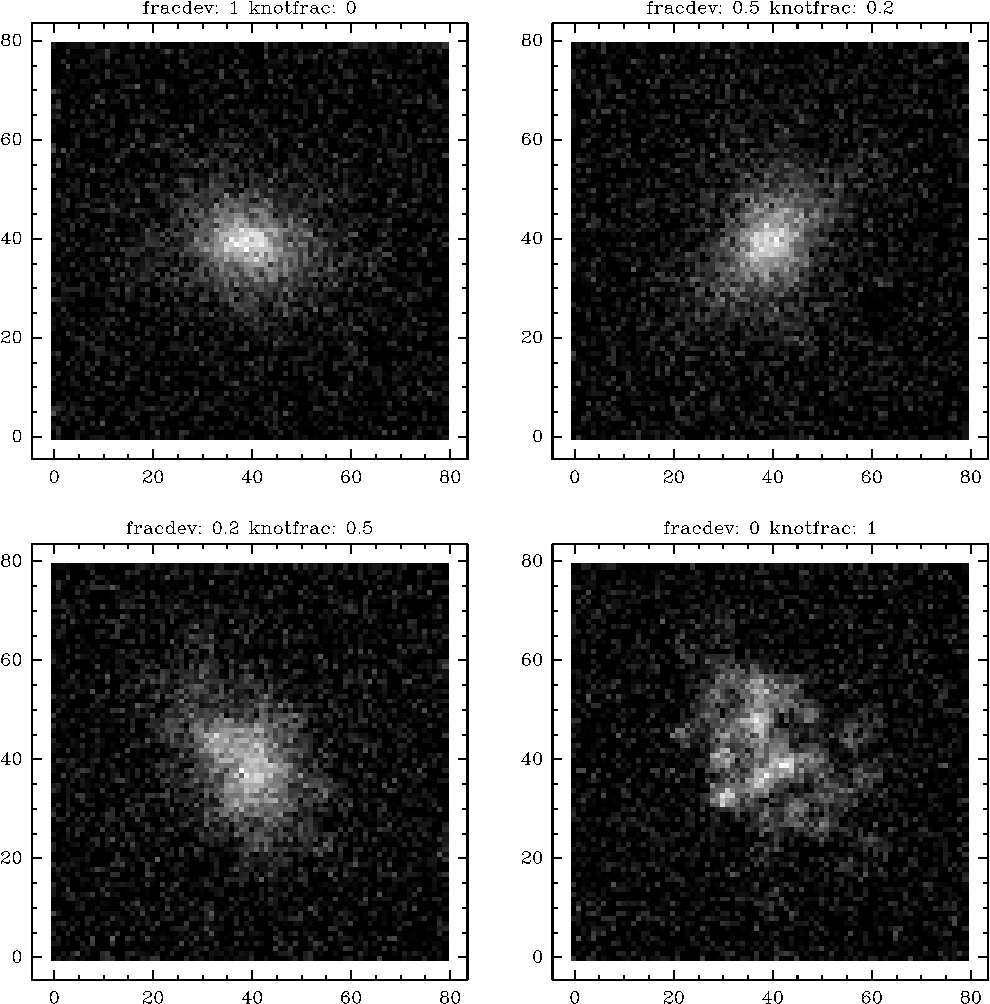
\includegraphics[width=0.7\textwidth]{mosaic-009086.pdf}
            \newline
        \end{center}

    }
    \setbeamertemplate{background canvas}[vertical shading][bottom=mgray,top=mblack]

}



\frame
{
    \frametitle{\snr}
 
    \begin{center}
        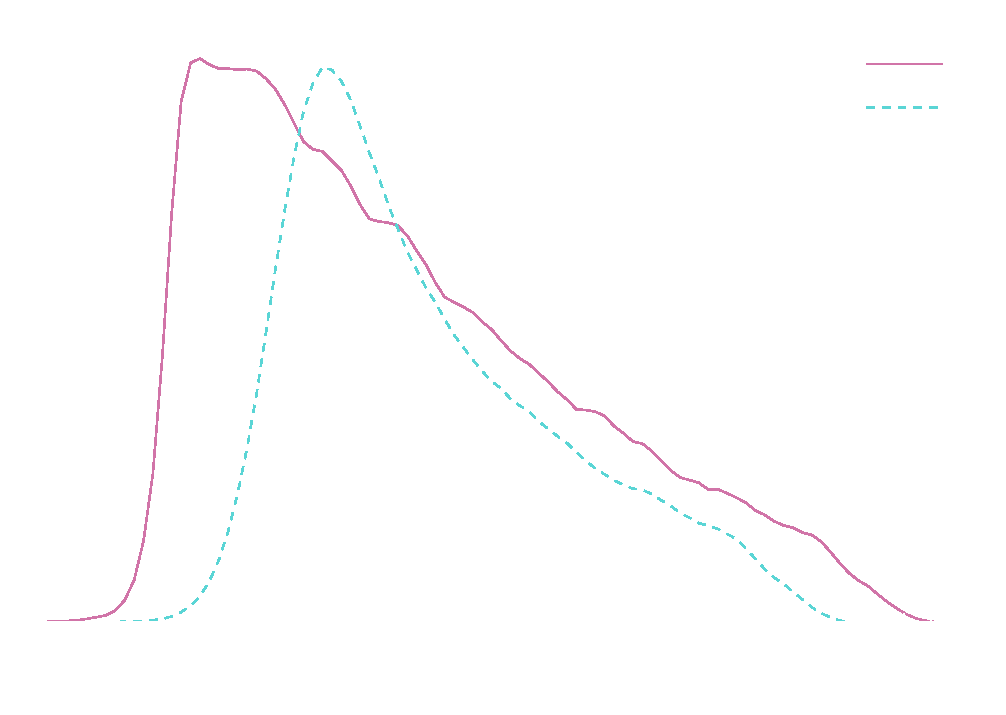
\includegraphics[width=\textwidth]{run-bdj03mcal01-s2n-inv.pdf}
        \newline
    \end{center}



}

\frame
{
    \frametitle{$r_{50}$}
 
    \begin{center}
        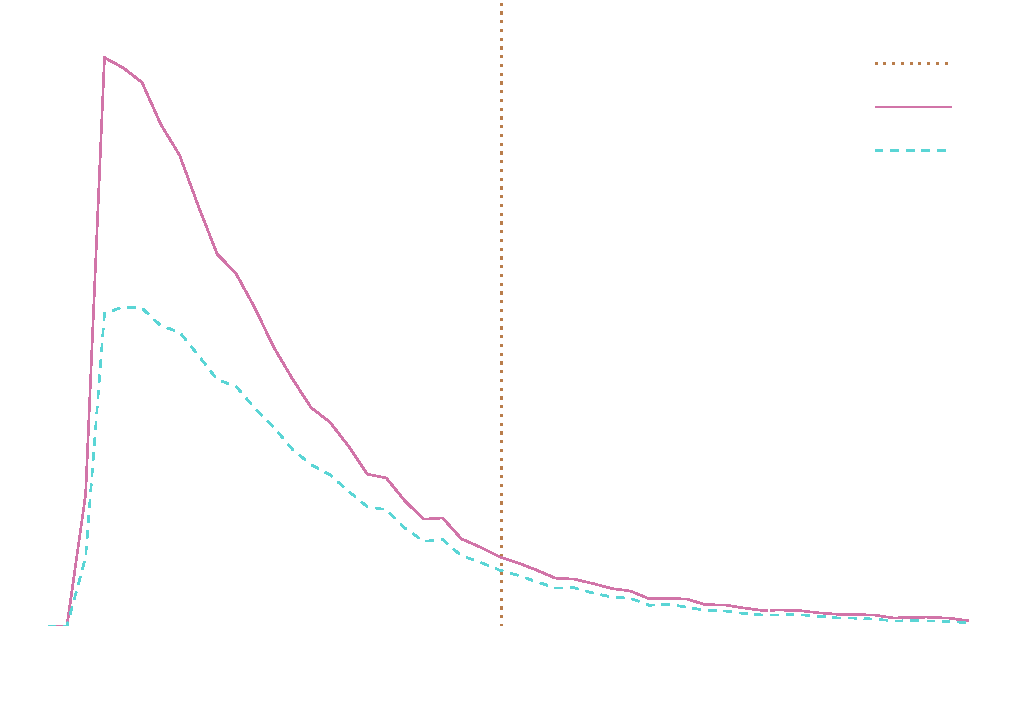
\includegraphics[width=\textwidth]{run-bdj03mcal01-r50-inv.pdf}
        \newline
    \end{center}



}



\frame
{
    \frametitle{\snr\ Cuts}
 
    \setbeamerfont*{itemize/enumerate body}{size=\Large}
    \setbeamerfont*{itemize/enumerate subbody}{parent=itemize/enumerate body}
    \setbeamerfont*{itemize/enumerate subsubbody}{parent=itemize/enumerate body}
 
    \begin{columns}
        \begin{column}{0.4\textwidth}
            \begin{itemize}
                \item Fitting {\color{lightsteelblue} adaptive moments} with 
                    {\color{red} no PSF correction}
                \item Select objects with \snr\ greater than some threshold.
            \end{itemize}
        \end{column}
        \begin{column}{0.6\textwidth}
            \begin{center}
            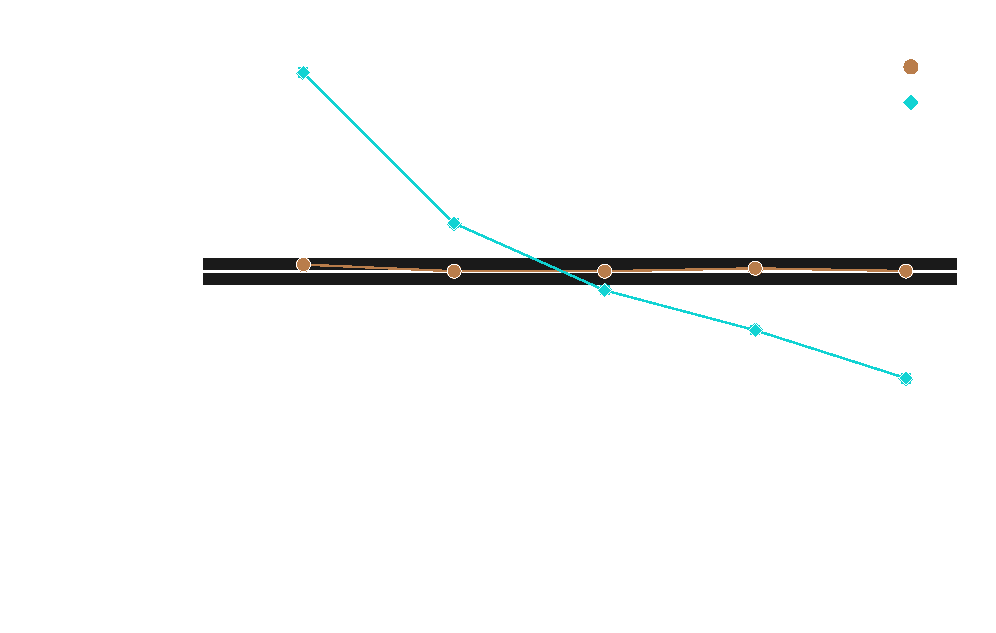
\includegraphics[width=\textwidth]{mc-select-bias-thresh-with-nocorr-inv.pdf}
                \newline
            \end{center}
        \end{column}
    \end{columns}


}

\frame
{
    \frametitle{\snr\ Cuts}
 
    \setbeamerfont*{itemize/enumerate body}{size=\Large}
    \setbeamerfont*{itemize/enumerate subbody}{parent=itemize/enumerate body}
    \setbeamerfont*{itemize/enumerate subsubbody}{parent=itemize/enumerate body}
 
    \begin{columns}
        \begin{column}{0.4\textwidth}
            \begin{itemize}
                \item Fitting {\color{lightsteelblue} adaptive moments} with 
                    {\color{red} no PSF correction}
                \item Select objects with \snr\ greater than some threshold.
            \end{itemize}
        \end{column}
        \begin{column}{0.6\textwidth}
            \begin{center}
            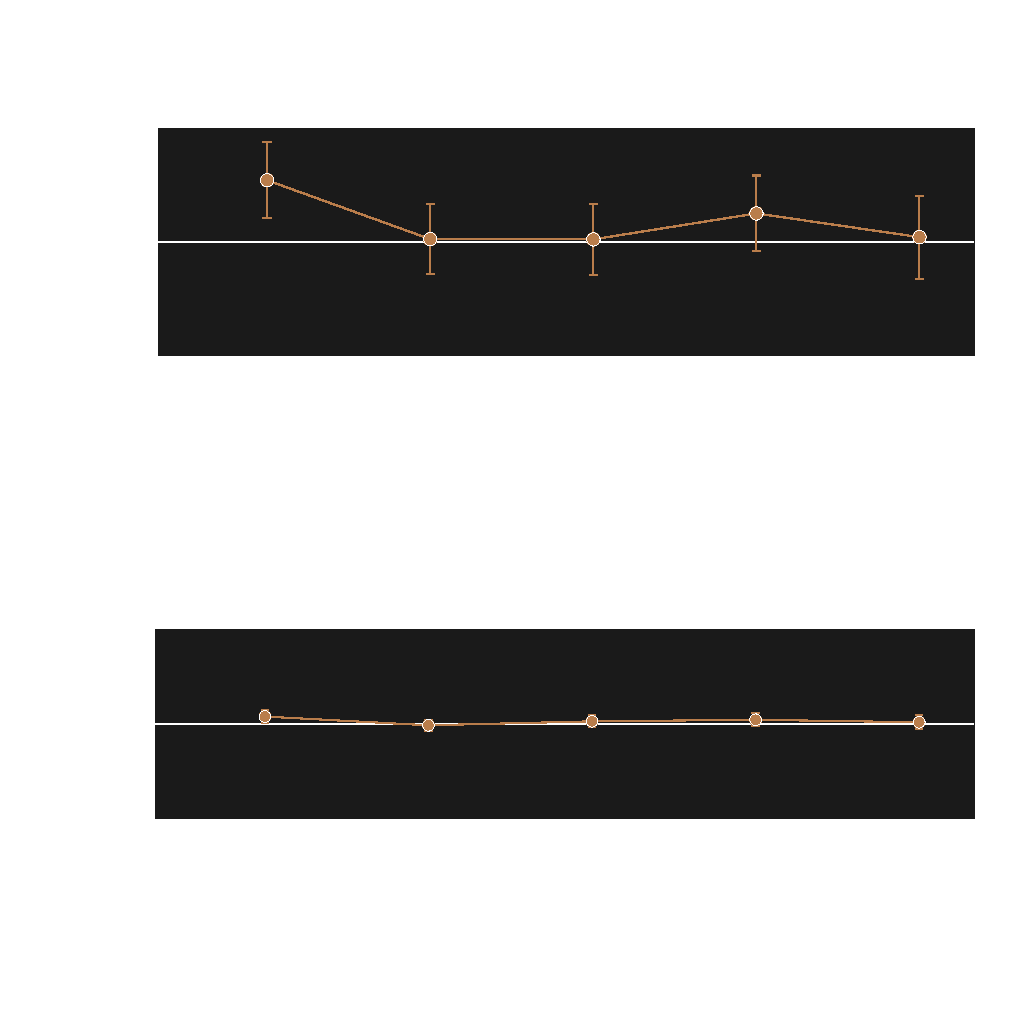
\includegraphics[width=\textwidth]{mc-select-bias-thresh-inv.pdf}
                \newline
            \end{center}
        \end{column}
    \end{columns}


}


\frame
{
    \frametitle{Summary}
    \begin{itemize}
        \item \Mcal\ is a new method for shear measurement.
            \begin{itemize}
                \item Does not require significant prior knowledge about galaxy properties.
                \item Correct for noise bias, model bias, and selection effects within 
                    the formalism.
                \item In challenging simulations, recover shear to accuracy required
                    for LSST
            \end{itemize}

        \item Two papers posted to the \texttt{arXiv} last week.
            \begin{itemize}
                \item Huff \& Mandelbaum \url{https://arxiv.org/abs/1702.02600}
                \item Sheldon \& Huff \url{https://arxiv.org/abs/1702.02601}
            \end{itemize}

        \item Using \mcal\ for shear measurement in the Dark Energy Survey.

    \end{itemize}
}




\end{document}
